%  To make a final copy of your thesis put a '%'
%  in front of the \includeonly command and run:
%    latex thesis
%    latex thesis
%    latex thesis
%    bibtex thesis
%    latex thesis
%    latex thesis
%
% See
%     http://www.ecn.purdue.edu/~mark/puthesis/#Options
% for documentclass options.

\documentclass[phys,miser,dissertation]{tuthesis}
% xzt
% figure
\graphicspath{{./figures/}}
\DeclareGraphicsExtensions{.pdf,.jpeg,.png}
\usepackage{graphicx}
\usepackage{balance}
\usepackage{subfigure}
\usepackage{float}
\usepackage{textcomp}
% \usepackage{caption}
%\usepackage{subcaption}
%\captionsetup[table]{format=plain,labelformat=simple,labelsep=period}
%\captionsetup[figure]{skip=0pt, labelformat=simple,labelsep=period}
%\subcaptionsetup[figure]{skip=0pt, labelsep=space}
\usepackage{indentfirst}
\usepackage{units}

% underline:
\usepackage{soul}

% algorithm
\usepackage[linesnumbered,ruled,vlined]{algorithm2e}
\usepackage{amsmath}
\usepackage{bbm}
\numberwithin{algocf}{chapter}
\SetKwInput{KwInput}{Input}                % Set the Input
\SetKwInput{KwOutput}{Output}              % set the Output
\usepackage{algcompatible}
\DeclareMathOperator{\atan2}{atan2}
\DeclareMathOperator{\clip}{clip}

% set the space in the algorithms and tables
\usepackage{setspace}
\usepackage{graphicx}
\usepackage{booktabs}
\usepackage{multirow}
\usepackage{placeins}
\usepackage{enumitem}
\newlist{abbrv}{itemize}{1}
\setlist[abbrv,1]{label=,labelwidth=1in,align=parleft,itemsep=0.1\baselineskip,leftmargin=!}
\def\RED{\color{black}}
\def\END{\color{black}}
\def\BLUE{\color{black}}
\usepackage{threeparttable}
\usepackage{amssymb}
\usepackage{mathrsfs} 
\usepackage{amsfonts,makecell}
%\setlength{\marginparwidth}{100pt}%
%\setlength{\textwidth}{410pt}
\usepackage[top=1in, bottom=1in, left=1.5in, right=1in, asymmetric]{geometry}

% *** ALIGNMENT PACKAGES ***
\usepackage{array}
\usepackage{tablefootnote}
\usepackage{makecell}

\usepackage{pdfpages}

% Maker sure hyperref is last becuase otherwise things get buggy!
% cite url websites: 
\usepackage[hyphens]{url}
\usepackage{hyperref}
\hypersetup{colorlinks=true,
            citecolor=black,
            linkcolor=black,
            urlcolor=black}
\usepackage{bookmark}


\newcommand{\ie}{\textit{i.e.,}\ }
\newcommand{\eg}{\textit{e.g.,}\ } % the \ ensures latex does not treat command as end of sentence

\DeclareMathOperator*{\argmax}{arg\,max}
\DeclareMathOperator*{\argmin}{arg\,min}
%-------------------------------------------------------------------
% Title of thesis (used on cover and in abstract).
% The title shown must be the full, official title of the thesis.
% Superscripts and subscripts are not permitted in the title.
% Reference: TM2006, page 26.
% Use \title{Put Title Here} for a one-line title.
% Use \\ to separate lines in multi-line titles.
% Put % at the end of the last line of a title
% to avoid getting an extra space in the abstract.
% There are two forms of title: one line or more than one line.
% There are examples of both below.
% Only use one \title.
% CHANGE NEXT FIVE LINES.
%\title{An Example Thesis Done with LaTeX}
%\title{%
%  An Example Thesis Done with LaTeX\\
%  that has a Very Long Title%
%}
\title{
\bfseries Robot Navigation in Crowded Dynamic Scenes}

% First author name with first name first is used for cover.
% Second author name with last name first is used for abstract.
% Your full name as it appears in the University records appears
% on the cover.
% Reference: TM2006 pages 26, 29.
% There are two forms of author, with and without initials.
% There are examples of both below.
% Only use one \author line.
% CHANGE NEXT TWO LINES.
\author{Zhanteng Xie}{Xie, Zhanteng}

% First is long title of degree (used on cover).
% Second is abbreviation for degree (used in abstract).
% Third is the month the degree was (will be) awarded (used on cover
% and in abstract).
% Last is the year the degree was (wlll be) awarded (used on cover
% and in abstract).
% The degree title for all doctoral candidates is ``Doctor of Philosophy''.
% The precise degree names for master's candidates appear in the list of
% ``Degrees Offered'' in the Graduate School bulletin.
% The date is the month and year that the degree is actually awarded.
% (If you have registered for ``degree only'', revise the thesis title
% page to reflect the new date on which the degree is to be awarded.)
% Reference: TM2006 pages 26--27, 30.
% CHANGE NEXT LINE?
\pudegree{DOCTOR OF PHILOSOPHY}{PhD}{August}{2024}

% Major professor
% Use, for example:
%     \majorprof{Sarah Smith}
%     \majorprof{Amy A. Jones}
%     \majorprofs{Sarah Smith and Amy A. Jones}
%     \majorprofs{Sarah Smith, Amy A. Jones, and Lisa B. C. Brown}
% depending on the number of major professors you have.
% CHANGE NEXT LINE.
\committee{
Philip Dames, Advisory Chair, Mechanical Engineering\\
Damoon Soudbakhsh, Mechanical Engineering\\
Daniel A. Jacobs, Mechanical Engineering\\
Xuesu Xiao, George Mason University\\
Iyad Obeid, External Reader, Electrical and Computer Engineering
}

% Campus (used only on cover)
% Use one of the following:
%     Philadelphia
% CHANGE NEXT LINE?
\campus{Philadelphia}

%
% My command definitions not specific to my thesis.
%
% \input{docs/mydefs}


% CHANGE NEXT TWO LINES?
% Let typing "\en" be exactly the same as typing "\ensuremath". 
\let\en=\ensuremath

% CHANGE NEXT TWO LINES?
% Set things up so \margins will show where the margins on the page are.
\newcommand{\margins}{\Repeat{Show where the margins for the page are.}{4}}

% CHANGE NEXT FIVE LINES?
% Define a \ve command with two arguments, so if it called with
%     \ve an
% it will expand to
%     {\en{a_1},~\en{a_2},\ \ldots,~\en{a_{n}}}
\newcommand{\ve}[2]{\en{#1_1},~\en{#1_2},\ \ldots,~\en{#1_{#2}}}

\usepackage{mathtools}
\DeclarePairedDelimiter\ceil{\lceil}{\rceil}
\DeclarePairedDelimiter\floor{\lfloor}{\rfloor}


% To LaTeX only some parts of your thesis put the
% names of the parts to include here.  For example,
% \includeonly{front} would only process front.tex.
% \includeonly{front,introduction} would only process
% front.tex and introduction.tex.
% To print the final copy of your thesis put a '%'
% in front of the \includeonly command and run LaTeX
% three times to make sure that all cross-references
% are correct.  Then run BibTeX once and LaTeX twice
% more.
% CHANGE NEXT LINE?
%\includeonly{front,introduction}
%\includeonly{front}

\makeindex

\begin{document}
% Start a new volume for your thesis.
% All theses must have at least one volume.
% If your thesis has multiple volumes put another "\volume"
% command between chapters below.
\volume
% Front matter:
% ABSTRACT
% DEDICATION
% ACKNOWLEDGMENTS
% PREFACE
% TABLE OF CONTENTS
% LIST OF TABLES
% LIST OF FIGURES
% LIST OF ILLUSTRATIONS
% CHAPTER #s AND TITLES
% NOTES
% BIBLIOGRAPHY/REFERENCES CITED
% APPENDIX LETTERS AND TITLES
%  This is ``front matter'' for the thesis.
%
%  Regarding ``References'' below:
%      KEY    MEANING
%      PU     ``A Manual for the Preparation of Graduate Theses'',
%             The Graduate School, Purdue University, 1996.
%      TCMOS  The Chicago Manual of Style, Edition 14.
%      WNNCD  Webster's Ninth New Collegiate Dictionary.
%
%  Lines marked with "%%" may need to be changed.
%
% \begin{copyrightpage}
%    %\vspace{1.8in}
%    \begin{center}
%       % xzt
%       \copyright \ Copyright 2024 By Zhanteng Xie\\
%    %\vspace{0.5cm}
%     % by\\
%    % \vspace{0.5cm}
%    % Firstname Lastname \\
%    % \vspace{-8pt}
%    % \noindent\rule{3.5cm}{0.4pt}\\
%    All Rights Reserved
%    \end{center}
% \end{copyrightpage}

% xzt:
\begin{copyrightpage}
    \begin{center}
      \copyright \\
      Copyright \\
      2024\\
       \vspace{0.5cm}
       by\\
       \vspace{0.5cm}
       Zhanteng Xie \\
       \vspace{-8pt}
       \noindent\rule{3.5cm}{0.4pt}\\
       All Rights Reserved
   \end{center}
\end{copyrightpage}

  % Abstract is required.
  % Note that the information for the first paragraph of the output
  % doesn't need to be input here...it is put in automatically from
  % information you supplied earlier using \title, \author, \degree,
  % and \majorprof.
  % Reference: PU 17.
\begin{abstract}
This is your abstract. 
\end{abstract}

  % Dedication page is optional.
  % A name and often a message in tribute to a person or cause.
  % References: PU 15, WNNCD 332.
\begin{dedication}
To your loved ones.
\end{dedication}

  % Acknowledgements page is optional but most theses include
  % a brief statement of apreciation or recognition of special
  % assistance.
  % Reference: PU 16.


\begin{acknowledgments}
To everyone who makes this happen. ``The night is darkest just before the dawn. But I promise you the dawn is coming." 
\end{acknowledgments}


  % The Table of Contents is required.
  % The Table of Contents will be automatically created for you
  % using information you supply in
  %     \chapter
  %     \section
  %     \subsection
  %     \subsubsection
  % commands.
  % Reference: PU 16.
\tableofcontents

  % If your thesis has tables, a list of tables is required.
  % The List of Tables will be automatically created for you using
  % information you supply in
  %     \begin{table} ... \end{table}
  % environments.
  % Reference: PU 16.
\listoftables

  % If your thesis has figures, a list of figures is required.
  % The List of Figures will be automatically created for you using
  % information you supply in
  %     \begin{figure} ... \end{figure}
  % environments.
  % Reference: PU 16.
\listoffigures

  % The preface is optional.
  % References: PU 16, TCMOS 1.49, WNNCD 927.
%\begin{preface}
%  This is the preface.
%\end{preface}

  % List of Symbols is optional.
  % Reference: PU 17.
%\begin{symbols}
%  $m$& mass\cr
%  $v$& velocity\cr
%\end{symbols}
%
%  % List of Abbreviations is optional.
%  % Reference: PU 17.
%\begin{abbreviations}
%  abbr& abbreviation\cr
%  bcf& billion cubic feet\cr
%  BMOC& big man on campus\cr
%\end{abbreviations}
%
%  % Nomenclature is optional.
%  % Reference: PU 17.
%\begin{nomenclature}
%  Alanine& 2-Aminopropanoic acid\cr
%  Valine& 2-Amino-3-methylbutanoic acid\cr
%\end{nomenclature}
%
%  % Glossary is optional
%  % Reference: PU 17.
%\begin{glossary}
%  chick& female, usually young\cr
%  dude& male, usually young\cr
%\end{glossary}

% this adds the blank space and "Chpater"  column required by the TUHB
\chapterscolumn


\chapter{Introduction}
% xzt: do not delete
\pagestyle{plain}

This is Level 1 heading: chapter 1.

\section{Overview}
This is Level 2 heading: section.

\section{Notations}
Throughout this dissertation, we use lower-case (upper-case) bold characters to denote vectors (matrices). 

\subsection{Formula}
This is Level 3 heading: subsection.

\subsubsection{Formula Example.}
This is Level 4 heading: subsubsection.

Equation~\eqref{eq:entropy} is an example from \cite{xie2024scope, xie2023stochastic} for placing an equation in the dissertation. 
\begin{equation}
        H(\bar{\mathbf{o}}) = -\frac{1}{N} \sum_{i=1}^{N}{\left[ \bar{\mathbf{o_i}} \log \bar{\mathbf{o_i}} + (1-\bar{\mathbf{o_i}}) \log (1 -\bar{\mathbf{o_i}}) \right]}.
        \label{eq:entropy}
\end{equation}
\chapter{Background}
% xzt: do not delete
\pagestyle{plain}

This is chapter 2.

\section{Figure}

Fig.~\ref{fig:navigation_examples} is an example from \cite{xie2024scope, xie2023drl, xie2023stochastic, xiao2022autonomous, chen2022semantic, xie2021towards} for placing a figure in the dissertation. For convenience, you can put the figures of one chapter in a single folder. 
  
\begin{figure}[t]
    \centering
    \subfigure[Simulated indoor environment]
    {
        \centering
        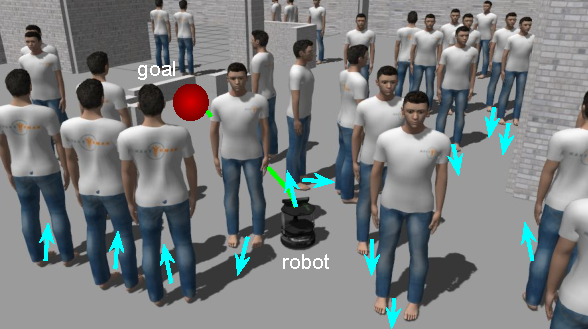
\includegraphics[width=0.77\linewidth]{figures/fig_gazebo_simulation_crowded.pdf}
        \label{fig:gazebo_navigation}
    } 
    %\vspace{0.01cm}
    \subfigure[Real-world outdoor environment]
    {
        \centering
        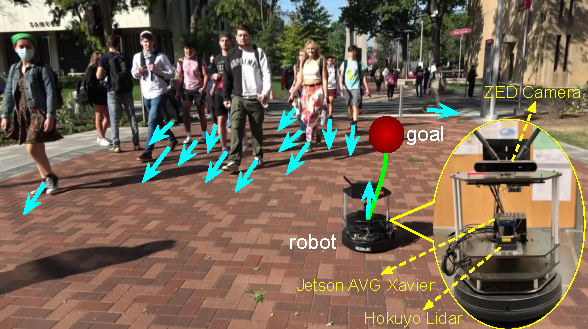
\includegraphics[width=0.77\linewidth]{figures/fig_real_world_outdoor.pdf}
        \label{fig:real_world_navigation}
    }%
     \bcaption[Illustration of the robot navigation problem.]{
    \ul{ Illustration of the robot navigation problem.}
     The robot navigates through crowds in a simulated indoor environment and a real-world outdoor environment. 
     The robot is following a nominal path (green line) to the goal (red disk) while avoiding pedestrians (blue arrows show current velocity).
    }
    \label{fig:navigation_examples}
\end{figure}





\chapter{Robot Perception}
% xzt: do not delete
\pagestyle{plain}

This is chapter 3. 

\section{Table}
Table~\ref{tab:fusion} is an example \cite{xie2023drl, xie2021towards} for placing a table in the dissertation.

\begin{table}[t]
    \setstretch{1.5}
    \centering
    \caption{Ablation experiment results with different fusion structures}
    \scalebox{0.85}{
        \begin{tabular}{c c c c c}
            \toprule
            \textbf{Network Structures} 
            & \textbf{RMSE} 
            & \textbf{EVA} 
            & \textbf{\# of Params} & 
            \textbf{FPS}\\
            \midrule
            
            Middle fusion  & \textbf{0.17} & \textbf{0.15} & \textbf{28.94 M} & \textbf{255.13} \\
            \midrule
            
            Late fusion  & 0.18 & 0.17 & 57.86 M & 140.53 \\
           \bottomrule
        \end{tabular}
    }
    \label{tab:fusion}
\end{table}



\chapter{Robot Prediction}
% xzt: do not delete
\pagestyle{plain}

This is chapter 4.

\section{Algorithm}

Algorithm~\ref{alg:gpu_mapping} is an example from \cite{xie2024scope, xie2023stochastic} for placing an algorithm in the dissertation.

\begin{algorithm}[t]
    \setstretch{1.5}
    \DontPrintSemicolon
    \caption{GPU-accelerated OGM mapping}
    \label{alg:gpu_mapping}
    
    \KwInput {compensated lidar measurements ${\mathbf{y}^R_{t-\tau:t}}$}
    \KwOutput {local environment map $\mathbf{m}$}
    
    \begin{algorithmic}[1]  
        \FORALL{time steps $n$ from $t-\tau$ to $t$}
            \FORALL{\textbf{parallel} grid cells $\mathbf{m}_i$ in the perceptual field of $\mathbf{y}^R_{n}$}    
            
            \STATE    $l_i = l_i + \log \frac{p(\mathbf{m}_i|\mathbf{y}^R_{n})}{1-p(\mathbf{m}_i|\mathbf{y}^R_{n})} - \log \frac{p(\mathbf{m}_i)}{1-p(\mathbf{m}_i)}$
            
            \ENDFOR 
        \ENDFOR
    \end{algorithmic}
\end{algorithm}
\chapter{Robot Navigation}
% xzt: do not delete
\pagestyle{plain}

This is Chapter 5.


	
	
\chapter{Robot Experiments}
% xzt: do not delete
\pagestyle{plain}

This is Chapter 6.	
\chapter{CONCLUSION}
% xzt: do not delete
\pagestyle{plain}

This is Chapter 7.
\chapter{FUTURE WORK}
% xzt: do not delete
\pagestyle{plain}

Good luck with your dissertation defense!
\bibliography{bib/template} 
%The files containing all the articles and books you ever referenced.

% Appendices are optional.
% Appendices are not necessarily a part of every thesis.
% An appendix is used for supplementary illustrative material,
% original data, computer programs, and other material that
% is not necessarily appropriate for inclusion within the
% text of your thesis.
% Reference: TM2006 page 33.
% Use "\appendix" for one appendix or "\appendices" for more than one
% appendix.
% CHANGE NEXT 7 LINES?
\appendix
\include{appendix}


%\include{demo-citations}
%\include{demo-figures}
%\include{demo-mathematics}
%\include{demo-multicols}
%\include{demo-tables}
%\include{demo-text}


% Notes and footnotes are optional.
% Reference: TM2006 page 34.
% I have not implemented this yet.  Mark Senn 2002-06-03
%%\include{notes}

% A vita is optional for masters theses
% and required for doctoral dissertations.
% Reference: TM2006 page 13.
% CHANGE NEXT LINE?
%\include{vita}

\end{document}

% LaTeX won't read after the \end{document} command.
% You can put notes to yourself or LaTeX input not
% ready for use here if you'd like.
